%----------------------------------------------------------------------------------------
%	CHAPTER
%----------------------------------------------------------------------------------------

\chapterimage{chapter_head_2.pdf} % Chapter heading image

\chapter{AGV commissioning}
In this chapter we will see how to setup the parameters of the AGVs in RDE environment. Before doing it, we will have a look on mechanical and electrical part of the controller.

%----------------------------------------------------------------------------------------
%
%----------------------------------------------------------------------------------------
\section{MGV mechanical and electrical part}
In this section we will describe one kind of AGV, that is MGV a  Magnetic guided vehicle. Some of the part of MGV are used in other king of AGVs. The difference is in the way of navigation and localization. The MGV have to follow a magnetic tap, using magnetic sensors. In this example the MGV use 4 magnetic sensors. Each magnetic sensor have 16 bits of output. The sensor is connected to a digital to canopen module in order to communicate with the controller.

In the middle of the MGV an RFID reader is placed. RFID cards are placed along the path on the magnetic tape, and are used as position feedback. The feedback is not continuous. 

Four motors and 4 drives are present. The drives take a velocity reference from the controller via analog signal, and send a velocity feedback from an encoder. The encoder signal is read in the controller via a high speed counter. Some digital IO are exchanged between controller and drive like drive reset, drive enable, drive ready or not in alarm, etc.

Steering is accomplished by modulating the speed of wheels. The angle of steering is relieved via a potentiometer, and read by the controller by an analog input module.

There are 2 laser scanner to monitor obstacles. Each laser scanner present 4 areas, that can be activated depending on the state of the AGV. Each area have 2 or 3 ranges of action. The fist one, smallest one, is used as a safety stop of the AGV. The senond range, middle, is used to slow down the AGV when the laser scanner detect some obstacle, and the third one is used as warning. Ther laser scanner have 4 digital inputs and 4 digital outputs.

The AGV is powered by a batteries.

The communication between the AGV and AgvManager is done via an Ethernet to wireless device. The device is configured as access point. And the Ethernet to wireless device in AgvManager is configured as client.

\begin{figure}[h]
	\centering
	\begin{subfigure}{0.4\textwidth}
		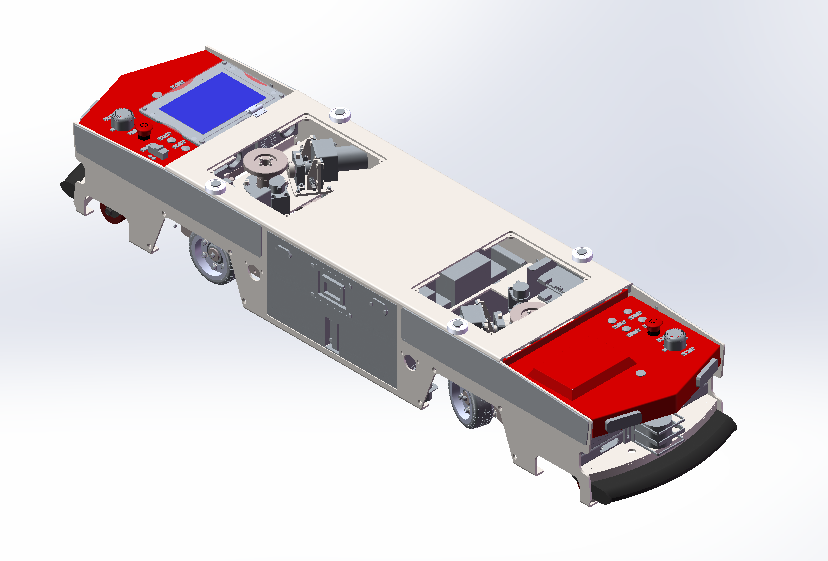
\includegraphics[width=\textwidth]{rde/agv/agvtop}
		\caption{Top view}
		\label{fig:agvtop}
	\end{subfigure}
	%\quad
	\begin{subfigure}{0.4\textwidth}
		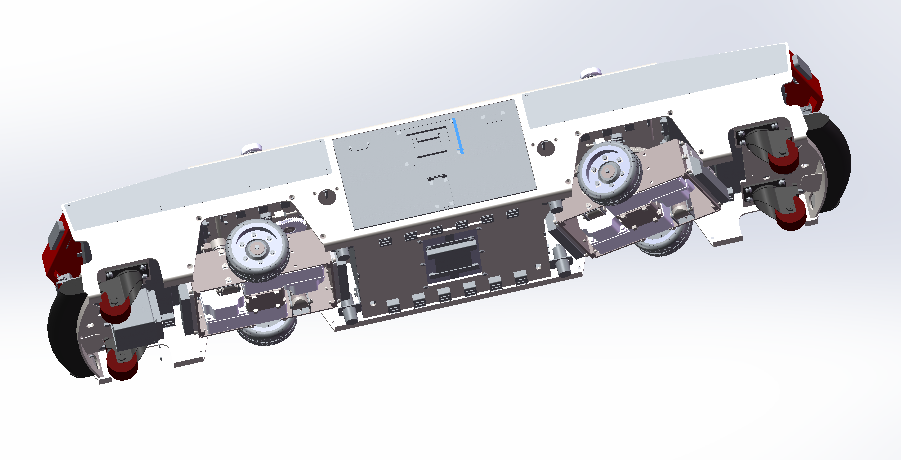
\includegraphics[width=\textwidth]{rde/agv/agvbottom}
		\caption{Bottom view}
		\label{fig:agvbottom}
	\end{subfigure}
	
	\begin{subfigure}{0.3\textwidth}
		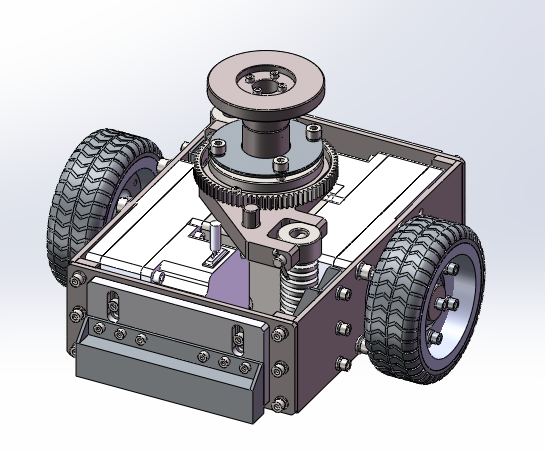
\includegraphics[width=\textwidth]{rde/agv/agvwheels}
		\caption{One set of wheels}
		\label{figagvwheels}
	\end{subfigure}
	\caption{Map line}\label{fig:agv}
\end{figure}

%----------------------------------------------------------------------------------------
%
%----------------------------------------------------------------------------------------
\section{Dispan : Display panel}


\begin{figure}[h]
	\centering
	\begin{subfigure}{0.4\textwidth}
	\centering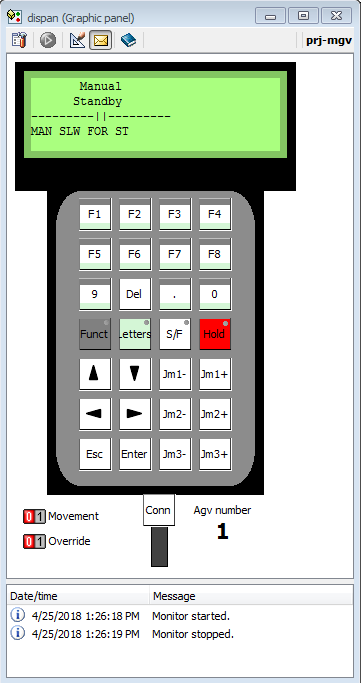
\includegraphics[scale=0.6, , angle =0]{rde/agv/dispanrde}
	\caption{Dispan in RDE Graphic panel}
	\label{figdispanrde}
	\end{subfigure}
	\quad
	\begin{subfigure}{0.4\textwidth}
	\centering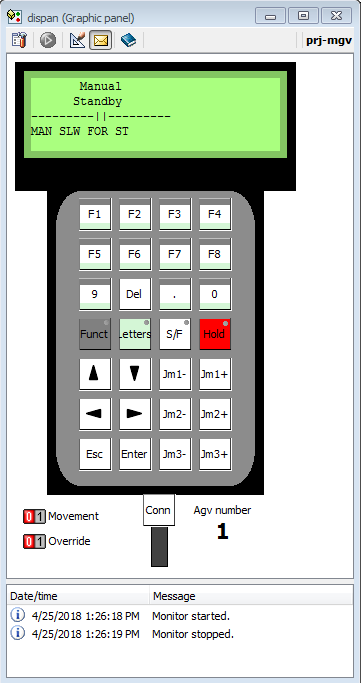
\includegraphics[scale=0.6, , angle =0]{rde/agv/dispanrde}
	\caption{Physical Dispan, communicate with the controller via RS485}
	\label{figdispanr}
	\end{subfigure}
\end{figure}
%----------------------------------------------------------------------------------------
%
%----------------------------------------------------------------------------------------
\section{Commissioning}
The first step in commissioning of any controller (plc or motion control) is to check the correct wiring of digital input and outputs. This step is relatively simple, using a variable monitor, online monitor or HMI we can debug the correct wiring of the signals following the electrical schematic.

Fig.\ref{fig:iosignals} show a template panel of IO signals for debugging purpose.
\begin{figure}[!]
	\centering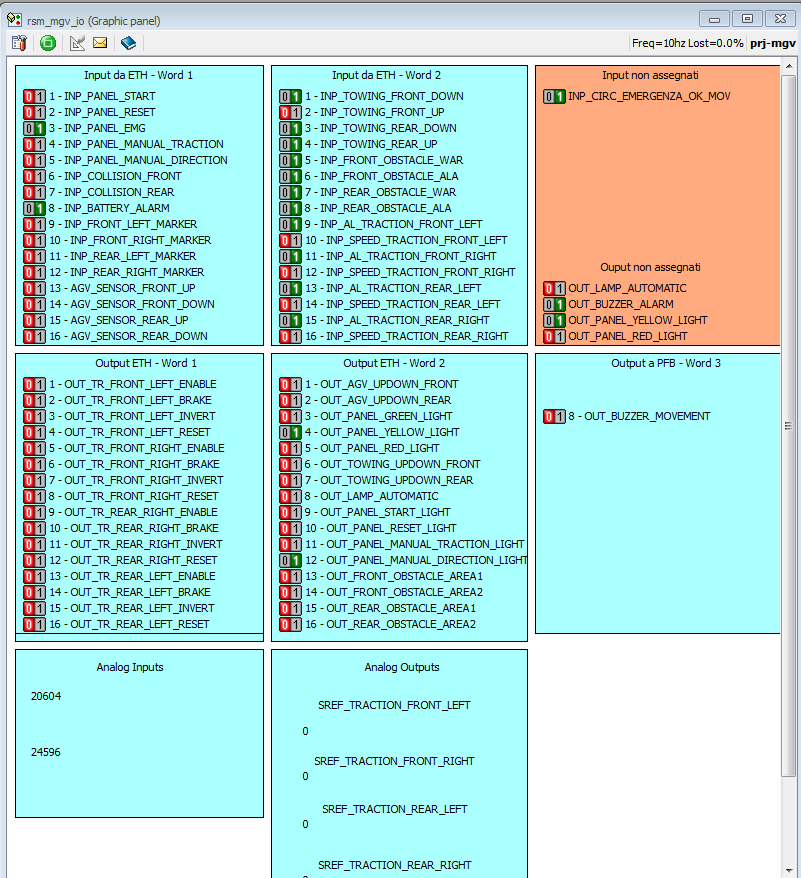
\includegraphics[scale=0.6]{rde/agv/iosignals}
	\caption{AGV IO signals. RDE graphic panel}
	\label{fig:iosignals}
\end{figure}

Once we are sure the electrical wiring is correct, we can proceed with tuning mechanical and eletrical components and software parameters.

%------------------
%
%------------------
\subsection{Potentiometer}
This AGV have 2 potentiometers, every one is connectes to a set of two wheels. When a the 2 wheels connected to the same mechanical axes, rotate with different speeds, the set of wheels wil rotate arround the center of the wheels coordinate system shown in fig.\ref{fig:agvwheelsystem}. The angle of rotation is measured via a potentiometer connected to the origin of the coordinate system via an elastic joint.

The potentiometer used in this AGV have a range between 0 and 270 degrees. The AGV can steer between $-30^{\circ}$ and $120^{\circ}$. We have to set the potentiometer in a way that the tension between pin 1 and 2 is around $3V$ when the wheels angle is at $0^{\circ}$.

After that we have to scale the analog input of the controller in order to read the correct angle. A linear relationship between the tension (or the raw value read by the analog input) an the angle in degree was supposed.

To adjust the parameters, we can use the dispan or a variable monitor. The procedure is to place the wheels at $0^{\circ}$ then at $90^{\circ}$ and read the corresponding value given by the analog input. Then assign the values to the variables \textcolor{blue}{NVRR\_POS\_0\_BIT\_SLEWING\_***} and \textcolor{blue}{NVRR\_POS\_90\_BIT\_SLEWING\_***}. Of course that same procedure have to be done for both potentiometers the front and the rear one fig.\ref{fig:agvwheelsystem}.

Using the dispan, we have to go to the voice F6 than choose 3 or 4 than save the parameters \figurename.\ref{fig:potDispanF}.

\begin{figure}[h]
	\centering
	\begin{subfigure}{0.4\textwidth}
		\centering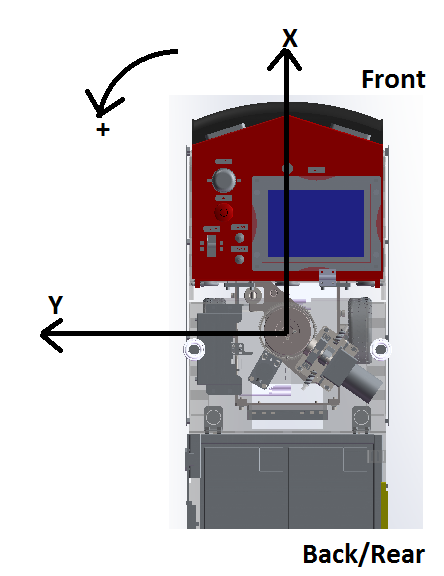
\includegraphics[scale=0.6, , angle =0]{rde/agv/agvtop2}
		\caption{AGV wheel coordinate system}
		\label{fig:agvwheelsystem}
	\end{subfigure}
	\qquad
	\begin{subfigure}{0.4\textwidth}
		\centering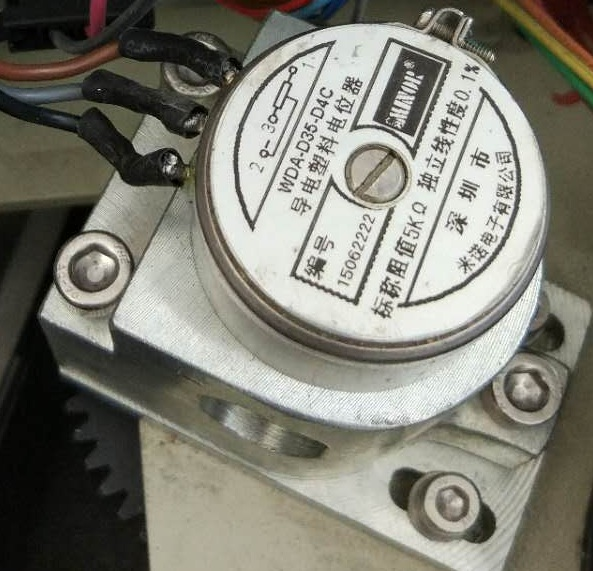
\includegraphics[scale=0.3, , angle =0]{rde/agv/potentiometer}
		\caption{Potentiometer connected to wheel vis an elastic joint}
		\label{fig:pot}
	\end{subfigure}
	
	\begin{subfigure}{0.4\textwidth}
		\centering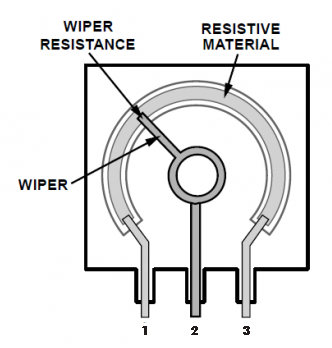
\includegraphics[scale=0.3, , angle =0]{rde/agv/potentiometer2}
		\caption{Potentiometer construction}
		\label{fig:pot2}
	\end{subfigure}
	\begin{subfigure}{0.4\textwidth}
		\centering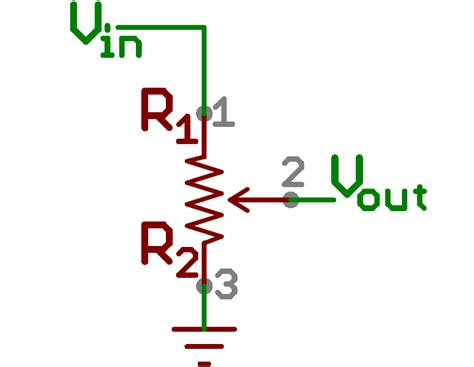
\includegraphics[scale=0.3, , angle =0]{rde/agv/potentiometersche}
		\caption{Potentiometer schematic}
		\label{fig:potschematic}
	\end{subfigure}
\end{figure}

\begin{figure}[h]
	\centering
	\begin{subfigure}{0.4\textwidth}
		\centering
		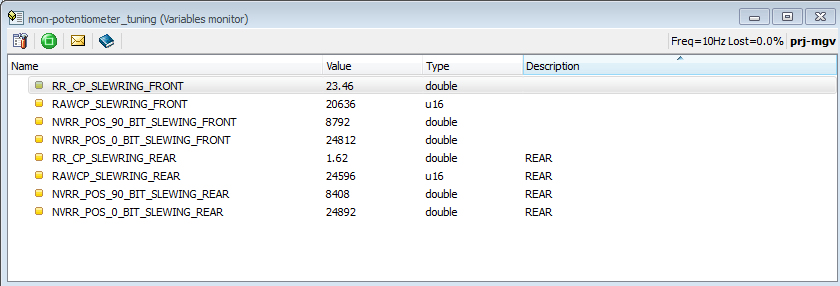
\includegraphics[scale=0.5]{rde/agv/potvarmonitor}
		\caption{RDE potentiometer variable monitor}
		\label{fig:potvarmonitor}
	\end{subfigure}

	\begin{subfigure}{0.4\textwidth}
		\centering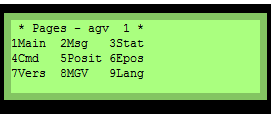
\includegraphics[scale=0.5]{rde/agv/dispanmain}
		\caption{Dispan main menu, reached by F1}
		\label{fig:dispanmain}
	\end{subfigure}
		\qquad
	\begin{subfigure}{0.4\textwidth}
		\centering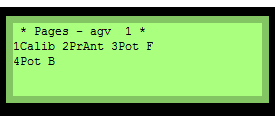
\includegraphics[scale=0.5]{rde/agv/dispanF6}
		\caption{Dispan 6Epos: Press 3 or 4 to tune the front or back potentiometer}
		\label{fig:dispanF6}
	\end{subfigure}
	\begin{subfigure}{0.4\textwidth}
		\centering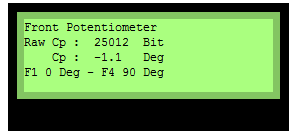
\includegraphics[scale=0.5]{rde/agv/dispanF6-3pot}
		\caption{Front potenziometer tuning. Turn the Wheels to 0 degree then press F1. Turn the wheels to 90 degree than press F4.}
		\label{fig:dispanF6-3pot}
	\end{subfigure}
	\label{fig::potprog}
	\caption{Potentiometer tuning}
\end{figure}

In lisiting.\ref{lstpotscale} is shown the code R3 that represent the relationship between the analog input and the angle in degree.

\begin{lstlisting}[caption= Scale potentiometer analog input, label=lstpotscale]
//	Read actual position of slewrings (steers)
// 	NVRR_POS_0_BIT_SLEWING_FRONT = Position of front slewing axis at 0 degrees in bits
// 	NVRR_POS_90_BIT_SLEWING_FRONT = Position of front slewing axis at 90 degrees in bits
//
if (NVRR_POS_0_BIT_SLEWING_FRONT <> NVRR_POS_90_BIT_SLEWING_FRONT)
	ScalaFront = 90.0 / (NVRR_POS_90_BIT_SLEWING_FRONT - NVRR_POS_0_BIT_SLEWING_FRONT)
	RR_CP_SLEWRING_FRONT = ScalaFront * (RAWCP_SLEWRING_FRONT - NVRR_POS_0_BIT_SLEWING_FRONT)
else
	RR_CP_SLEWRING_FRONT = 999.9		// Error
endif

if (not range(CP(AX_SLEWRING_FRONT), MIN_STR(AX_SLEWRING_FRONT), MAX_STR(AX_SLEWRING_FRONT)))
	alarm_set(AL_WHEEL_RANGE, AX_SLEWRING_FRONT)
endif
//
// 	NVRR_POS_0_BIT_SLEWING_REAR = Position of rear slewing axis at 0 degrees in bits
// 	NVRR_POS_90_BIT_SLEWING_REAR = Position of rear slewing axis at 90 degrees in bits
;
if (NVRR_POS_0_BIT_SLEWING_REAR <> NVRR_POS_90_BIT_SLEWING_REAR)
	ScalaRear = 90.0 / (NVRR_POS_90_BIT_SLEWING_REAR - NVRR_POS_0_BIT_SLEWING_REAR)
	RR_CP_SLEWRING_REAR = ScalaRear * (RAWCP_SLEWRING_REAR - NVRR_POS_0_BIT_SLEWING_REAR)
else
	RR_CP_SLEWRING_REAR = 999.9		// Error
endif

if (not range(CP(AX_SLEWRING_REAR), MIN_STR(AX_SLEWRING_REAR), MAX_STR(AX_SLEWRING_REAR)))
	alarm_set(AL_WHEEL_RANGE, AX_SLEWRING_REAR)
endif
\end{lstlisting}
%------------------
%
%------------------
\subsection{Magnetic sensors and Canopen modules}
The 16 bits magnetic sensors are connected to canopen modules. Address have to be given to canopen modules, this can be done using the dispan and connecting every module to the \textcolor{red}{CAN2} port of the controller, and the address is given one by one to the modules.

The figure fig.\ref{fig:antprg} show the steps of the procedure.

\begin{figure}[h]
	\centering
	\begin{subfigure}{0.4\textwidth}
		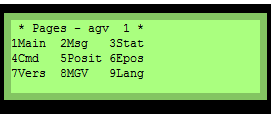
\includegraphics[scale=0.5]{rde/agv/dispanmain}
		\caption{Dispan main menu, F1}
		\label{fig:dispanmain1}
	\end{subfigure}	
	\begin{subfigure}{0.4\textwidth}
		\centering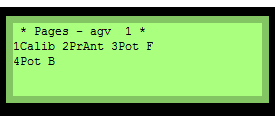
\includegraphics[scale=0.5]{rde/agv/dispanF6}
		\caption{Dispan F6 menu}
		\label{fig:dispanF613}
	\end{subfigure}
	
	\begin{subfigure}{0.4\textwidth}
		\centering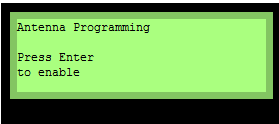
\includegraphics[scale=0.5]{rde/agv/dispanF6-2Ant}
		\caption{From F6 menu, press 2, to open the 2PrAnt page. Press enter to confirm}
		\label{fig:dispanF614}
	\end{subfigure}
	\begin{subfigure}{0.4\textwidth}
		\centering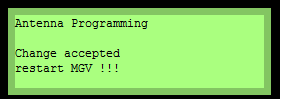
\includegraphics[scale=0.5]{rde/agv/dispanF6-2Ant2}
		\caption{Restart AGV}
		\label{fig:dispanF615}
	\end{subfigure}
	\begin{subfigure}{0.4\textwidth}
		\centering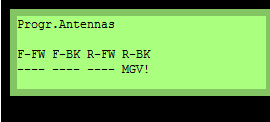
\includegraphics[scale=0.5]{rde/agv/dispanF6-2Ant3}
		\caption{After restarting AGV we can connect the canopen module to program them. When finsh press MGV to terminate and restart the AGV.}
		\label{fig:dispanF616}
	\end{subfigure}
	\caption{Magnetic sensor canopen programming}
\label{fig:antprg}
\end{figure}

%------------------
%
%------------------
\subsection{Laser scanner}
Every laser scanner have 4 inputs and 4 outputs. These digital signals are 4 bit code to identify the active area and the requested area. In our example we use only two input and two outputs.

The model of laser scanner we use, have 16 areas. The binary code is shown in fig.\ref{fig::laserscannerobstacle}.

\begin{figure}[!]
	\centering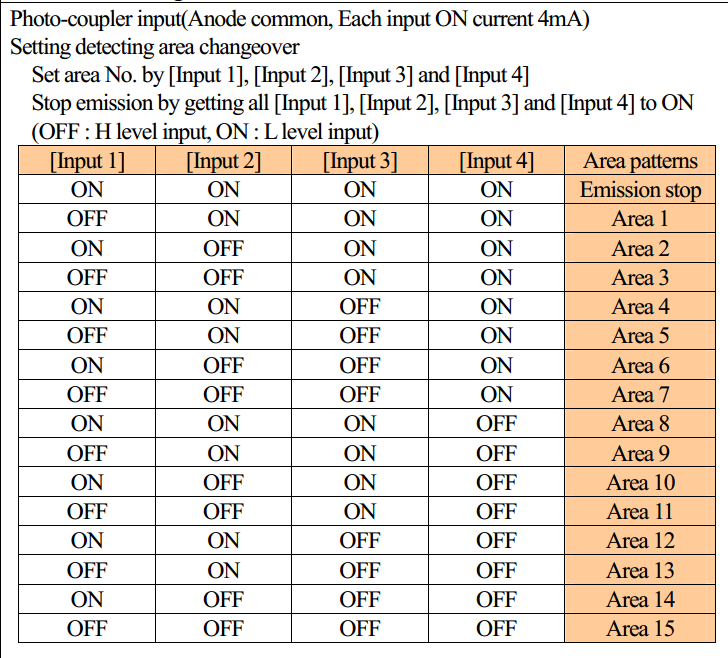
\includegraphics[scale=0.5]{rde/agv/laserscanner-pbs}
	\caption{PBS-03JN laser scanner area code}
	\label{fig:laserscannerpbs}
\end{figure}

Four different areas will be defined depending on the state of the agv. For example if the agv is not moving the alarm range of the 2 laser scanner should be extremely small. If the AGV is going forward the range of the front laser scanner should be bigger than the rear lase scanner and viceversa. We can define also another range for curving depending on the position of fixed obstacles.

Areas are activated using the digital inputs of the laser scanner (controller outputs). Following the codification of the laser scanner model e.g. fig.\ref{lstlaser}.

\begin{figure}[h]
	\centering
	\begin{subfigure}{0.4\textwidth}
		\centering
		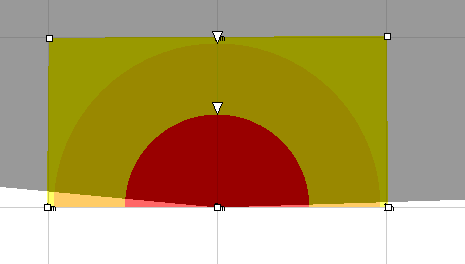
\includegraphics[scale=0.5]{rde/agv/laserscannerbigarea}
		\caption{Laser scanner area with big alarm range}
		\label{fig:laserscannerbigarea}
	\end{subfigure}
	
	\begin{subfigure}{0.4\textwidth}
		\centering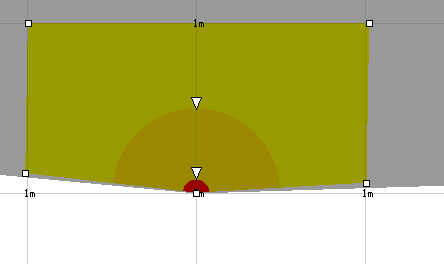
\includegraphics[scale=0.5]{rde/agv/laserscannersmallarea}
		\caption{Laser scanner area with small alarm range. Active when AGV is not moving.}
		\label{fig:laserscannersmallarea}
	\end{subfigure}
	\qquad
	\begin{subfigure}{0.4\textwidth}
		\centering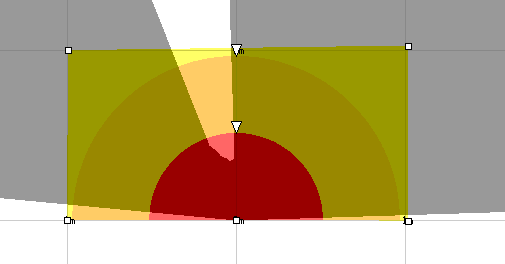
\includegraphics[scale=0.5]{rde/agv/laserscannerobstacle}
		\caption{Laser scanner area, obstacle detected in the alarm area. AGV will stop moving.}
		\label{fig:dispanF6}
	\end{subfigure}
	\label{fig::laserscannerobstacle}
	\caption{Laser scanner areas}
\end{figure}

\subsection{AGV parameters}
In task 1, AGV parameters file is loaded, the file name is written in register nvsr(1) NVSR\_PLANT\_CONFIG\_FILE, by calling the function LoadAgvConfig(). We can create a parameter file called "params-rsm.stp" and assign the register nsvr(1) with file name.

In the parameter file we can find, the name of the map to be used, mechanical parameters listing.\ref{lstmecparam}, etc.

\begin{lstlisting}[caption=params-rsm.stp Mechanical paramter of the AGV, label=lstmecparam]
;
;	Registers for mechanical configuration
;
rr(100)	0.4185				; RR_POS_SLEWRING_STEER_FRONT_X	[m] X position of the center of the front slewring
rr(101) 0.0					; RR_POS_SLEWRING_STEER_FRONT_Y	[m] Y position of the center of the front slewring
rr(102) 0.1525				; RR_RADIUS_SLEWRING_FRONT		[m] Distance from the center of the wheel composing the electronic front steer
rr(103)	-0.4185				; RR_POS_SLEWRING_STEER_REAR_X	[m] X position of the center of the rear slewring
rr(104) 0.0					; RR_POS_SLEWRING_STEER_REAR_Y	[m] Y position of the center of the rear slewring
rr(105) 0.1525				; RR_RADIUS_SLEWRING_REAR		[m] Distance from the center of the wheel composing the electronic rear steer
\end{lstlisting}

\subsection{Register backup}
Non volatile registers are stored in memory, when RTE is loaded it retrieve the values from the memory. It is a good idea anyway to backup the values of non volatile registers to a file, and load them in case of loss of memory.

We can save the values of registers to a file by sending the command \textcolor{red}{uar /fb/lostreg.stp}. The file lostreg.stp is a file which contain desired register to be saved. For example if we want to save only the values of regiters nvrr(140) and nvrr(162) we write in the file only these. When calling the command uar, only these registers are saved. There is a template file that can be used as a starting point.

If RTE lose memory, it load the file /fa/lostreg.stp when needed, the operator have to confirm it. In the file /fa/lostreg.stp there is a link to the file /fb/lostreg.stp.

For example if we have more than one agv, with different register values, we can call the command uar for each agv then copy the file /fb/lostreg.stp to our computer, e.g. \textcolor{red}{fsave -o /fb/lostreg.stp agv01/lostreg.stp} , this command copy the file from /fb to the folder agv01 in the project directory.

\subsection{General definitions}
Variables defined globally, at project level fig.\ref{fig:generaldefinitions}.
\begin{figure}[h]
	\centering
	\begin{subfigure}[h]{0.4\textwidth}
		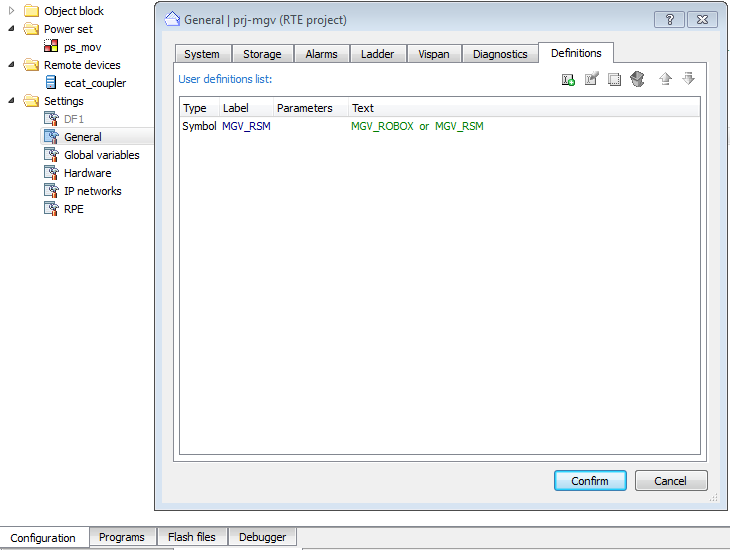
\includegraphics[scale=0.5]{rde/agv/generaldefinitions}
		\caption{Variable definitions, project level}
		\label{fig:generaldefinitions}
	\end{subfigure}
	
	\begin{subfigure}[h]{0.4\textwidth}
		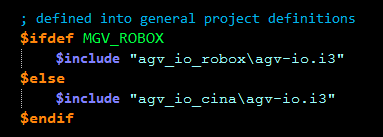
\includegraphics[scale=0.5]{rde/agv/generaldefinitions2}
		\caption{If the variable MGV\_ROBOX is defined gloably, a file is included otherwise another one is included.}
		\label{fig:generaldefinitions2}
	\end{subfigure}
	\label{fig:generaldefinition}
	\caption{Global variable definitions}
\end{figure}

%----------------------------------------------------------------------------------------
%
%----------------------------------------------------------------------------------------
\section{AGV ecosystem}

%------------------
%
%------------------
\subsection{Software and tools}
The software needed to program and setup an AGV are:
\begin{enumerate}
	\item Map generator : RAT can be used
	\item AgvManager : Script and path planning
	\item Compilers: RCE and ICmap compilers
	\item RDE
	\item Database : optional \\
\end{enumerate}

The electronic hardware needed:
\begin{enumerate}
	\item RP1 : Robox controller to control AGV
	\item personal computer: Where AgvManager will be executed
	\item Plc or RP1: As an interface with signals from the plant
	\item Wireless switch to communicate between RP1 and AgvManager
\end{enumerate}

%------------------
%
%------------------
\section{AgvManager-RP1 communication protocol}


%----------------------------------------------------------------------------------------
%
%----------------------------------------------------------------------------------------
\section{Hardware configuration}

%----------------------------------------------------------------------------------------
%
%----------------------------------------------------------------------------------------
\section{Program description}
The Agv program consist of 2 RTE projects: AGV program and antenna program. The antenna program is used only to program the address of canopen devices. The AGV program is used to control the agv and communicate with AgvManager.

The agv program is written in R3 and in Object blocks. The R3 program consist of 7 tasks and one Rule. And the OB program consist of 2 object blocks: one for wheel control, with 2 instances, and one for AGV with one instance. The ob for Agv is changed depending on the type of the agv. In this example we will use the mgv object block for magnetic guided vehicles.

Some logic is written in R3 other logic is written in OB. Important non volatile parameters are saved in the file \textcolor{red}{lostreg.stp}, this file is used as backup in case the memory of the agv is lost.

We already see how to set some parameters and value in RDE or in the dispan. AGV operations changes from plant to plant. The main logic, a part from improvements, still the same. Plant specific logic changes. These kinds of operations, that the AGV get from AgvManager have to be implemented in R3.

For example, if we need to implement the logic of the LOAD command operation from AgvManager we have to do it in \textcolor{blue}{rules--> function eseguiOperazioni()}. The constant O\_LOAD have to be defined in the file \textcolor{blue}{operations.i3}. The value of the constant should be equal to the value defined in AgvManager, that is 2.



